                               %----------------------------------%
                               % Manhattan College Math Dept      %
                               % Student Homework Template v1     %
                               %    R. Goldstone, 1/1/2011        %
 	               % Edited by T. McGrail, 2/11/2011  %
 	               % Edited by R. McGovern, 8/16/2011 %
 	               % Edited by J. Kirtland, 1/20/2015 %
                               %----------------------------------%
% PREAMBLE ============================================================================

\documentclass[12pt]{article}
\usepackage[utf8]{inputenc}    % set input encoding so bullets are printed
\usepackage{amssymb,amsmath,amsthm}
\usepackage{listings}
\usepackage[usenames,dvipsnames]{color}
\usepackage{matlab-prettifier}
\usepackage{graphicx}

 
% FILL-IN, THEN GO TO DOCUMENT MAIN BODY **********************************************
% TEXWORKS: USE CTRL-TAB TO JUMP FROM INPUT FIELD TO INPUT FIELD
\newcommand{\myname}{Amy Pitts} % Enter name
\newcommand{\duedate}{March 13, 2019} % Enter date, e.g., April 1
\newcommand{\courseno}{440L}      % Enter course number (just the number)
\newcommand{\coursename}{Machine Learning}    % Enter course name
\newcommand{\instructorname}{Instructor: Dr. Pablo Rivas} % Enter instructor name
\newcommand{\assignumber}{Midterm}   % Enter assignment number#.
\newcommand{\exerciselist}{Midterm}      % Enter problem references.  Give a complete list, in order, of all of the problems that you will do on this assignment.  Use the format 2.20 to designate problem  # 20 from chapter 2 of the text.
\newcommand{\spacingfactor}{2}
% END FILL-IN *************************************************************************

% DOCUMENT STRUCTURES -----------------------------------------------------------------

% PAGES
\usepackage[paper=letterpaper, margin=1in, headsep=20pt]{geometry}
  
\newcommand{\firstpageinfo}  
    {\textsf{\large\myname}    \hfill     Math \courseno{:}\,\coursename \\
  Assignment Number \assignumber \hfill  Due:  \duedate \\
  \instructorname}
% END PAGES

% HEADERS AND FOOTERS
\usepackage{fancyhdr}
\pagestyle{fancy}              % Headers and footers for page 2 and beyond
  \lhead{\textit{\myname}}
  \chead{\textit{Math \courseno}}
  \rhead{\textit{\textit{Assignment Number \assignumber}}}
  \cfoot{\textit{\thepage}}
  \renewcommand{\headrulewidth}{0.4pt}
% END HEADERS AND FOOTERS

% TEXT SPACING
\usepackage{setspace}   %Allows for Doublespacing
\usepackage{ifthen}   %Used to create a response environment
% END TEXT SPACING

% PROBLEM AND RESPONSE ENVIRONMENTS
 \newcommand\myqed{}                 % creates command for tombstone at end of proof
\newcommand{\printmyqed}[1][]       % decides whether to print tombstone or not
  {%
  \ifthenelse{\equal{#1}{Proof}}
  {\renewcommand{\myqed}{\qed}}
  {\renewcommand{\myqed}{}}
  }

\newenvironment{exercise}[1][]{%
  \bigskip                          % Space before problem statement
  \noindent \textsf{Exercise #1.}\slshape }{}
   
\newenvironment{response}[1][\textit{Solution}]{%
  \printmyqed[#1]
  \begin{spacing}{\spacingfactor}
  \medskip                          % Space before solution
  \noindent \textit{#1.}}{\myqed\end{spacing}\medskip\hrule}
% END PROBLEM AND RESPONSE ENVIRONMENTS

% =====================================================================================

\begin{document}
\thispagestyle{empty}

% TOP MATTER --------------------------------------------------------------------------
\noindent\firstpageinfo
\begin{center} \underline{\textsf{Exercise List}}\\[5pt] \exerciselist \end{center}
\medskip\hrule
% END TOP MATTER ----------------------------------------------------------------------


%----------------------------------------------------------------------------------------


\begin{exercise}[1] % Put problem reference inside the brackets
  Compare two algorithms on a classification task: the Pocket 
  algorithm (designed for classification), and linear regression 
  (not designed for classification). For linear regression, after 
  learning the weights $w$; ; we use $h(x) = sign(w^T x)$ to 
  classify $x$. For the dataset, start by using the following 
  Python code: In file labeled $midterm_generate.py$ \\
  Create another dataset using the same method as above but now 
  you will classify between 4 and the rest of the numbers. 
  To do this you should change lines 8 and 9 as follows: 
  $y[y<>4] = -1$ \\ $y[y==4] = +1$ \\
  Try the following three approaches using the dataset with 
  the new changes, plot the final (best) hypothesis on each 
  and then explain which works best in terms both Eout and the 
  amount of computation required. E.g., what is the final 
  classification error? after how many iterations did you stop 
  the Pocket algorithm?
  \begin{enumerate}
    \item[a)] The Pocket algorithm, starting from $w = 0$
    \item[b)] Linear regression (applied as a classification method).
    \item[c)] The Pocket algorithm, starting from the solution given by linear regression  
  \end{enumerate}
\end{exercise}
   
\begin{response}[Solution] 
  \textbf{a)}
    The number of iterations is 29 with a final classification 
    error of 6182. \\
    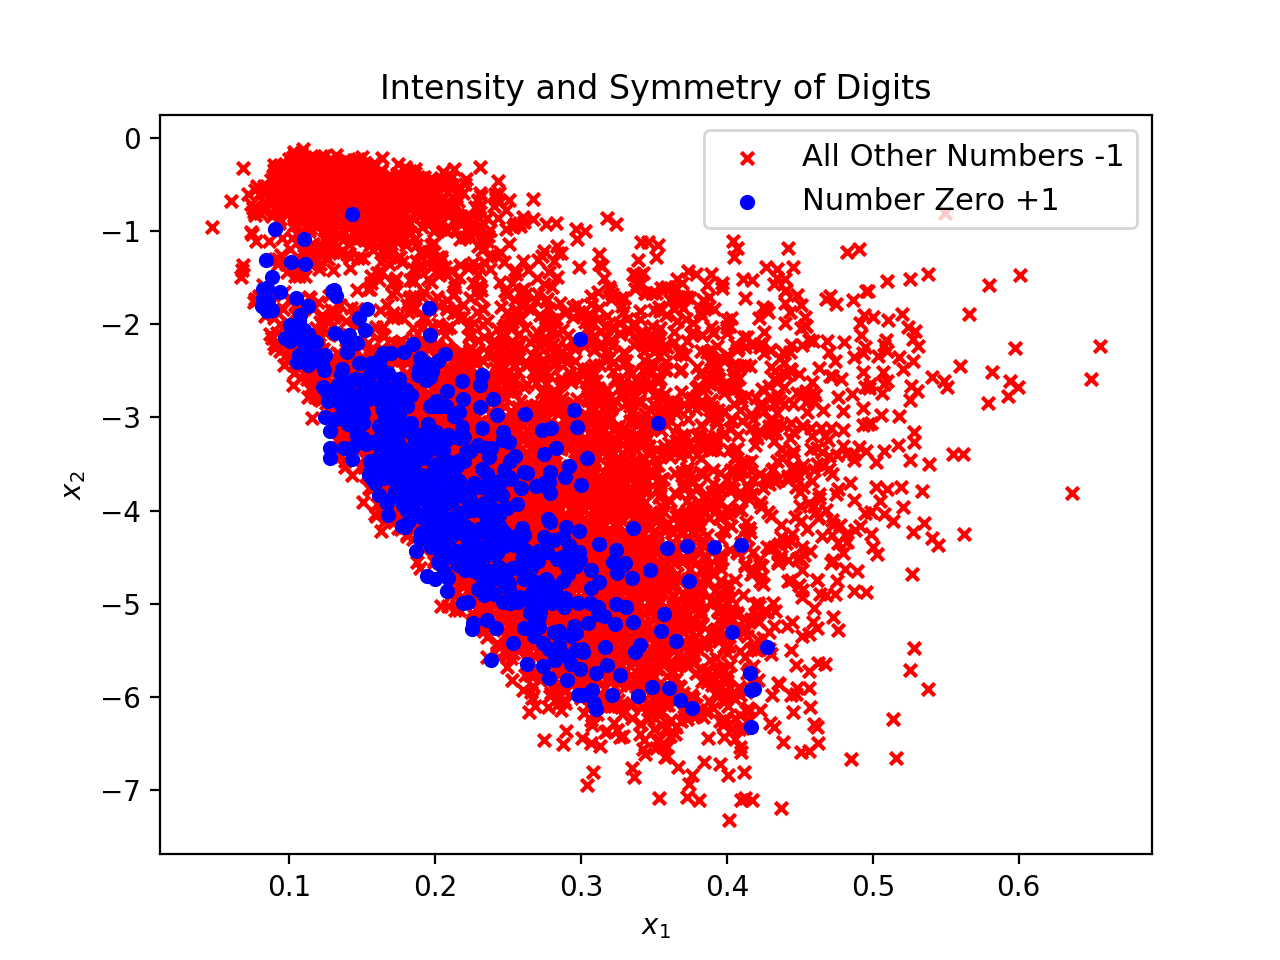
\includegraphics[width=85mm]{pics/a_original.png}
    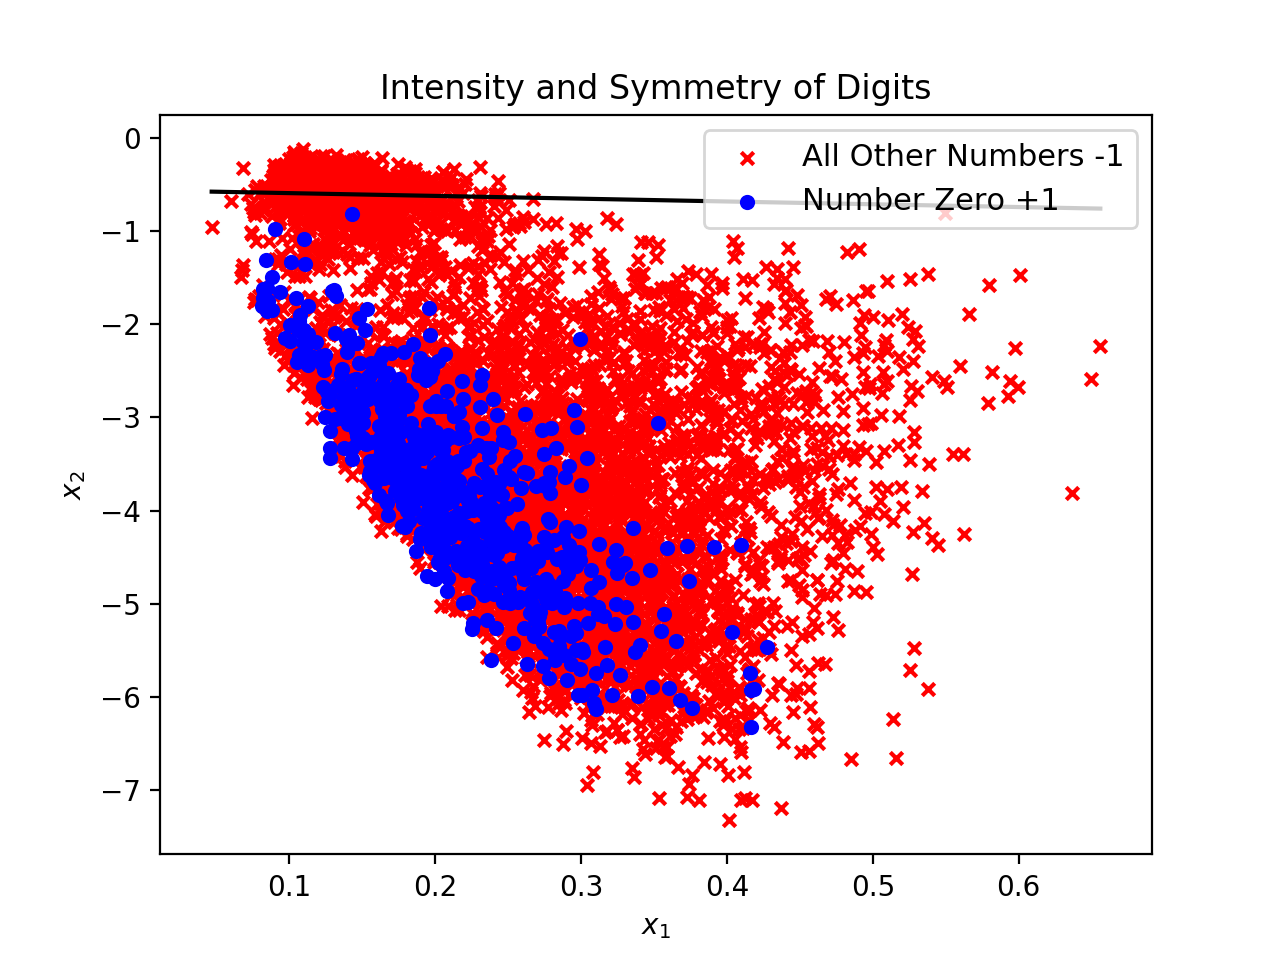
\includegraphics[width=85mm]{pics/a_fit.png} 
    
    \textbf{b)}
    This was just plotting the linear regression on the 
    data so there was no iterations.  \\
    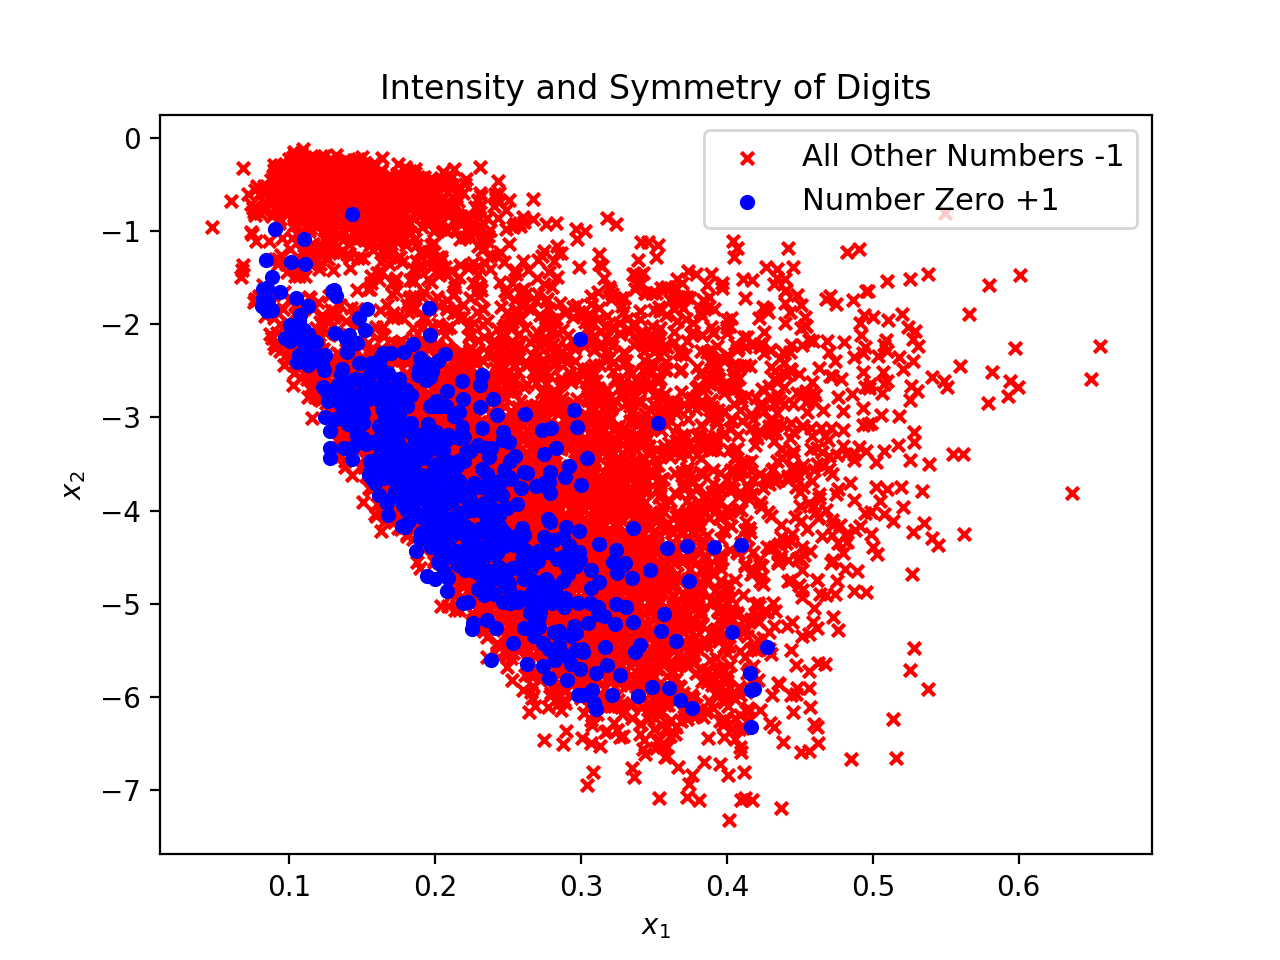
\includegraphics[width=85mm]{pics/b_original.png}
    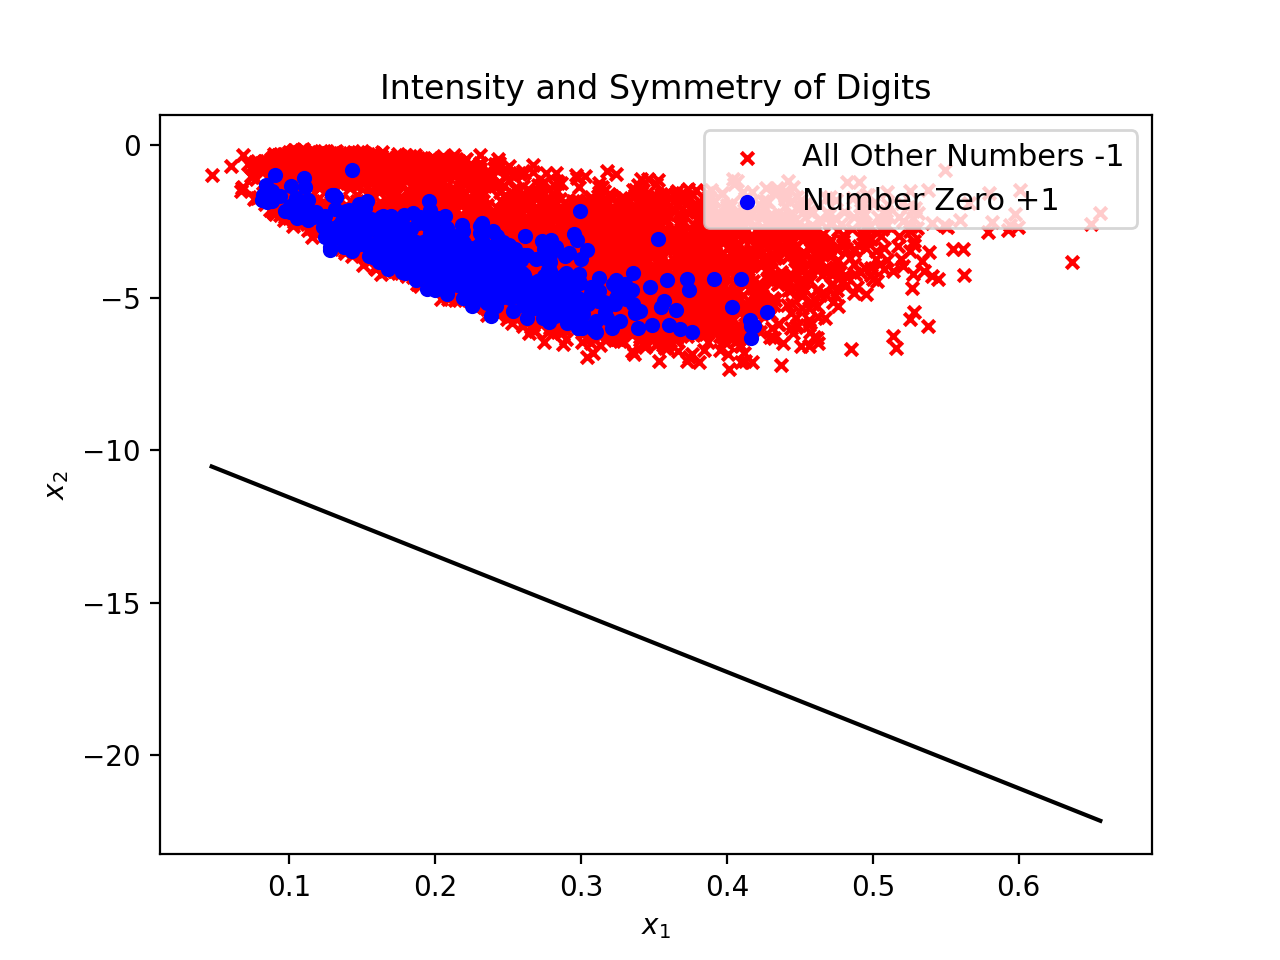
\includegraphics[width=85mm]{pics/b_fit.png} 
    
    \textbf{c)}
    The number of iterations is 29 with a final classification 
    error of 652. \\
    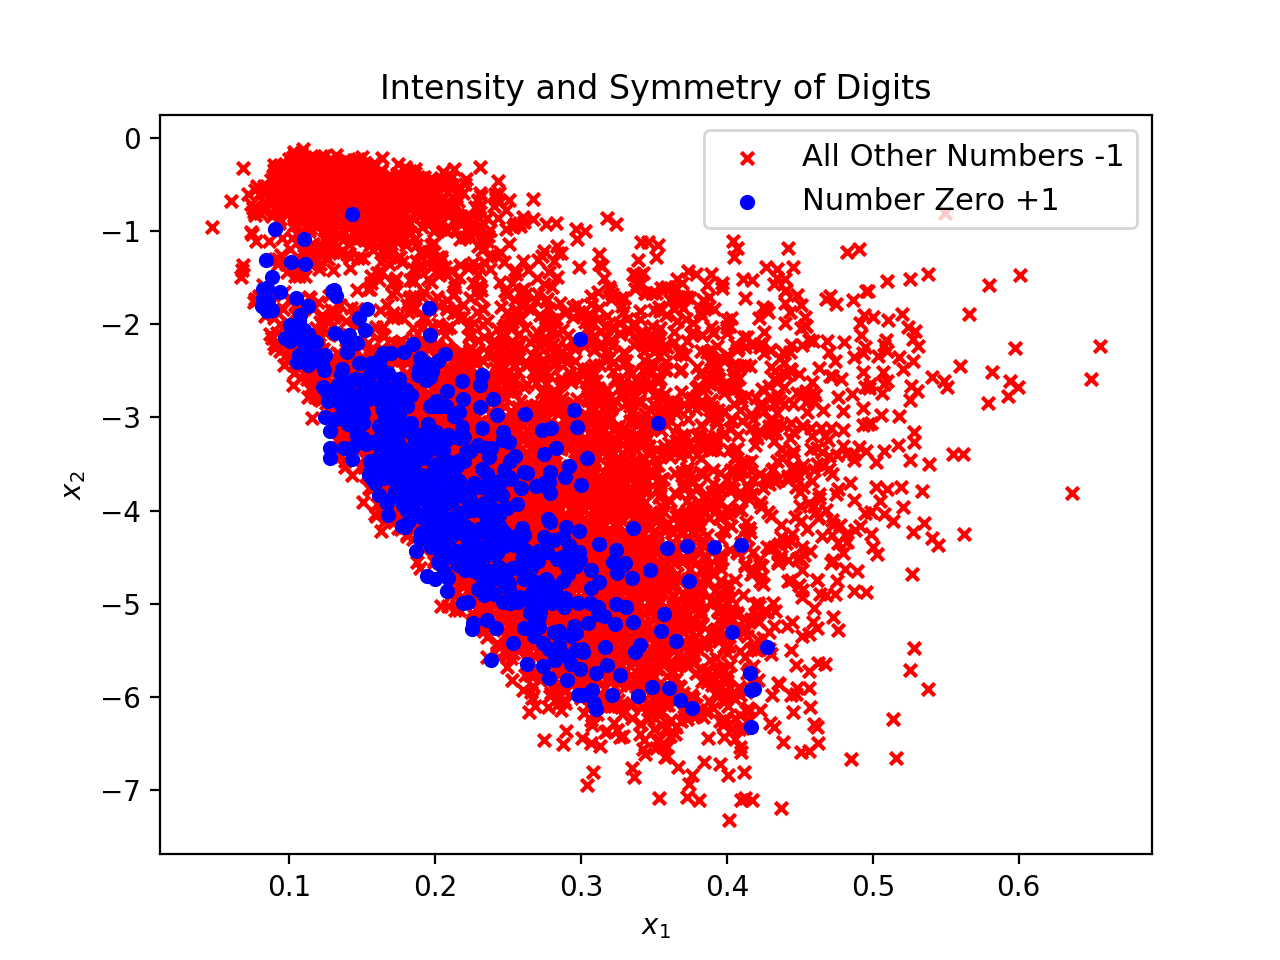
\includegraphics[width=85mm]{pics/c_original.png}
    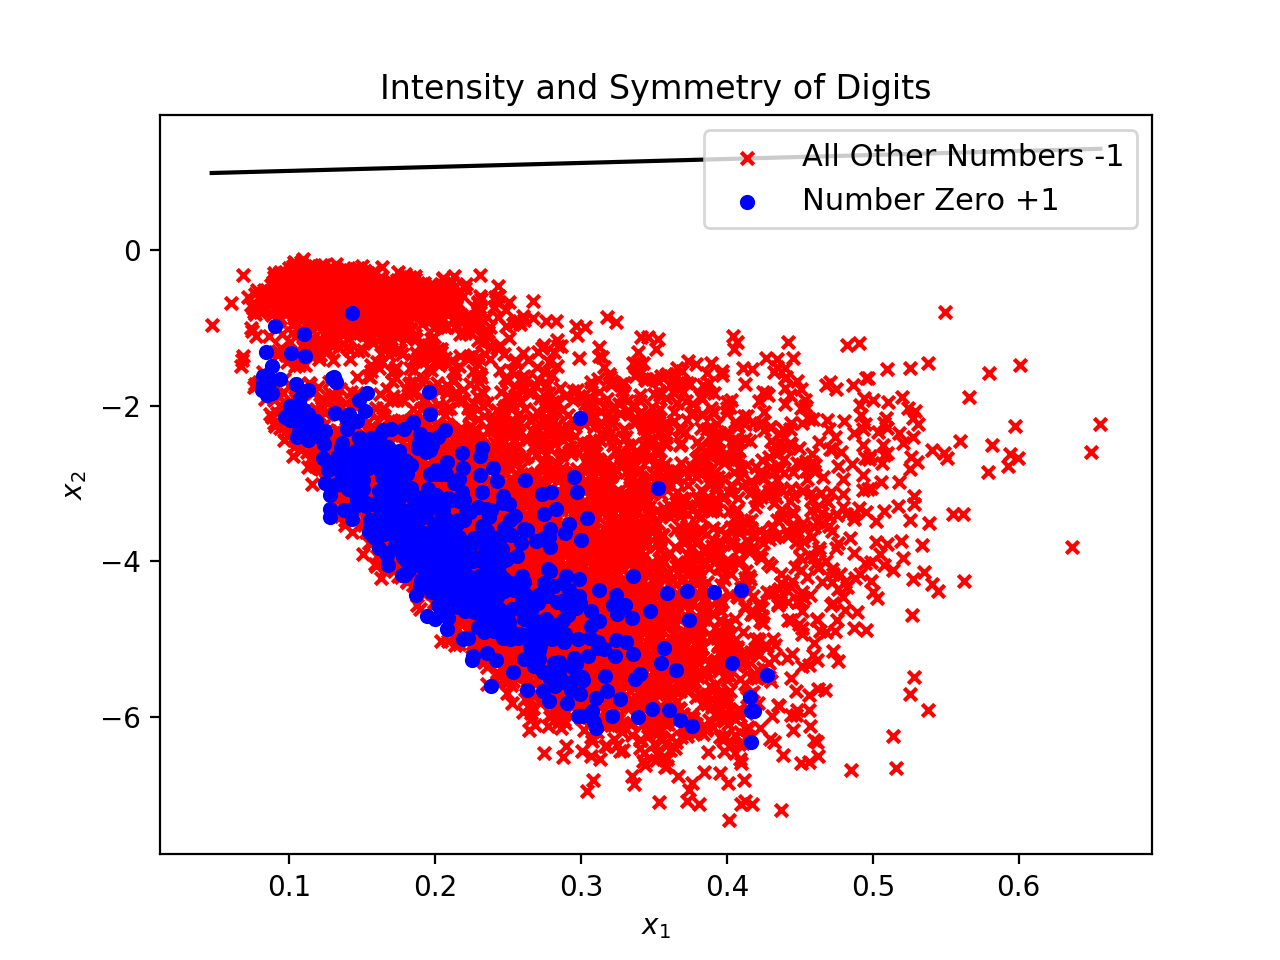
\includegraphics[width=85mm]{pics/c_fit.png} 
    
    \textbf{Summary:} The linear regression produced a lower 
    classification error but the graph itself does not make a 
    whole lot of sense. This might be because in another dimensionality 
    or with the line as a plane it would split the data in a way to 
    classify 4. The code for this question is in q1.py. 
      
\end{response}


%------------------------------------------------------

\begin{exercise}[2] % Put problem reference inside the brackets
  Write a Python program that solves \textbf{Problem 2.12 }in an iterative manner. 
  If you are feeling adventurous, plot the values of N as the 
  program converges to a steady value of N. \\
  \textbf{Problem 2.12: } For an $H$ with $d_{VC}=10$, what sample size do you need 
(as prescribed by the generalization bound) to have a 95\% confidence
that your generalization error is at most 0.05? 
\end{exercise}
   
\begin{response}[Solution] 
  Using the equation $N \geq \frac{8}{\epsilon^2}\ln \left(\frac{4((2N)^{d_{vc}}+1)}{\delta}\right)$
  and plugging in we have 
  \begin{align*}
    N &\geq \frac{8}{\epsilon^2}\ln \left(\frac{4\left((2N)^{d_{vc}}+1\right)}{\delta}\right) \\
    &= \frac{8}{0.05^2}\ln \left(\frac{4(2N)^{10}+4}{0.05}\right) \\
    &= 3200\ln \left(81920N^{10}+80\right)
  \end{align*}
  We want to find the $N$ which makes the equation true.
  We start with an initial seed of 20000. It does not mater 
  what seed we start with, it will converge to the fixed point.  
 \lstinputlisting[language=Python,frame=single]{python/q2.py}
  Using the code above the optimal number for $N$ is 
  452957 rounding up when comparing 8 decimal places.
  Below is the graph of the values of N against the iteration. 
  The graph starts at a low value of 20000 and then it levels 
  of as it approaches 452957. \\
  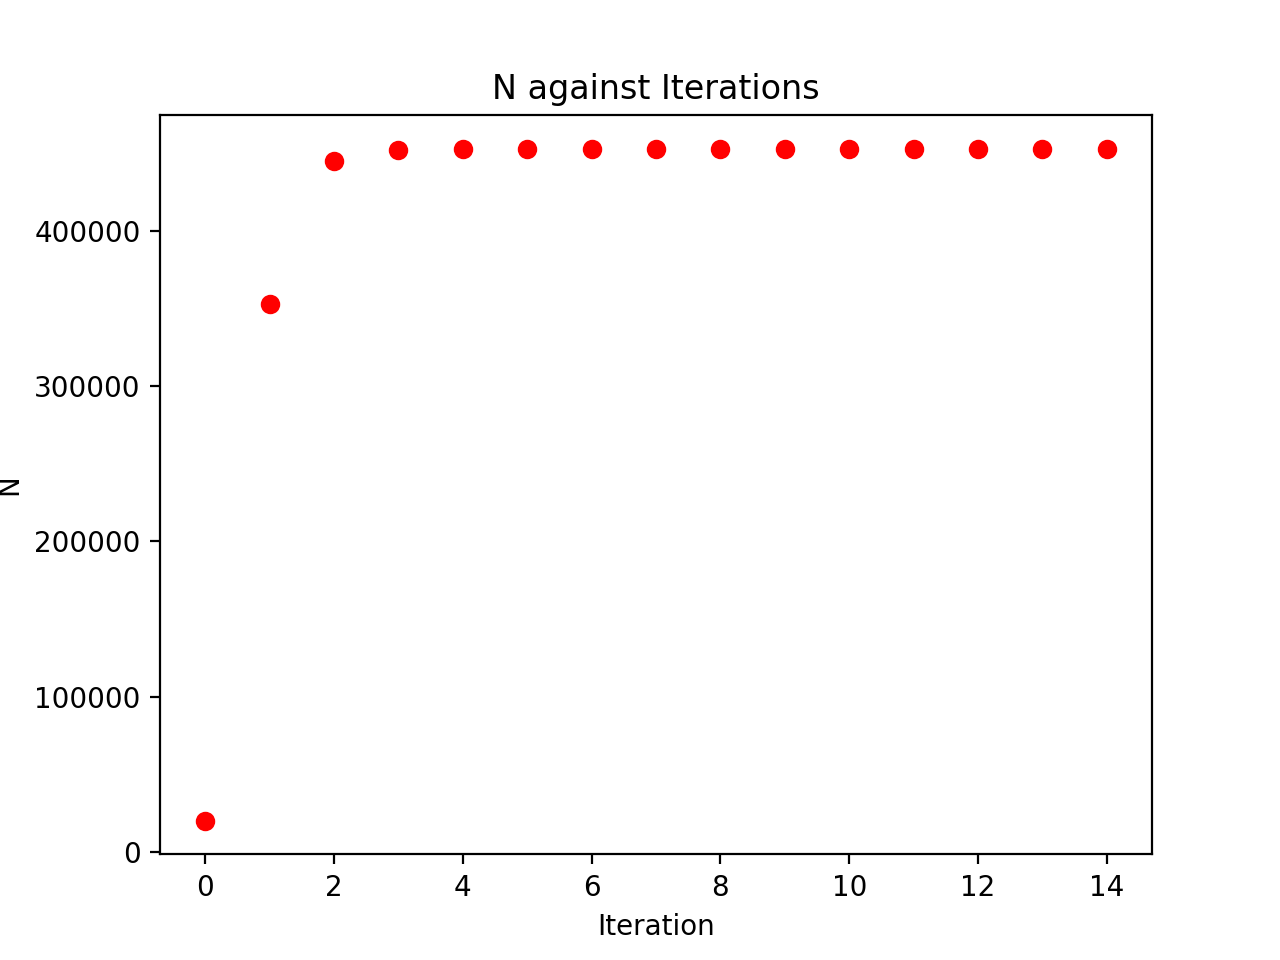
\includegraphics[width=150mm]{pics/q2_N.png} 
\end{response}

%------------------------------------------------------

\begin{exercise}[3] % Put problem reference inside the brackets
  (Extra Credit) Albert Einstein said “Creativity is intelligence 
  having fun”. You are very smart and talented. That is why you 
  are in this class. With that in mind... I recently acquired the 
  domain name $marist.ai$ and I am looking to create site for 
  students and faculty to share their AI-related projects;
  so, for a chance to be displayed our future website, draw some 
  type of logo for the new site here:
\end{exercise}
   
\begin{response}[Solution] \\
  
\includegraphics[width=150mm]{pics/logo.jpg} 
\end{response}


\end{document}
%======================================================================================
% END DOCUMENT MAIN BODY ==============================================================
% COPY AND PASTE THIS DOUBLE-SPACE PROBLEM-RESPONSE PAIR AS NEEDED
%======================================================================================



